\documentclass[10pt,a4paper]{moderncv}
\moderncvtheme{banking}
\moderncvcolor{blue}
\moderncvstyle[]{banking}

\usepackage[T1]{fontenc}
\usepackage{inputenc}
\usepackage[margin=1.8cm]{geometry}
\usepackage[sfdefault, light]{roboto}

% Customizations

\makeatletter

\newcommand\intlphone[2]{
  \def\@intlphonenumber{#2}
  \def\@intlphonelink{#1}
}
\newcommand\github[1]{\def\@github{#1}}
\newcommand\linkedin[1]{\def\@linkedin{#1}}
\newcommand\coversubject[1]{\def\@coversubject{#1}}

\definecolor{darkchocolate}{HTML}{323031}
\definecolor{subtlegrey}{HTML}{666265}
\definecolor{lightgrey}{HTML}{999891}
\definecolor{deepseablue}{HTML}{084C61}
\definecolor{algeabloom}{HTML}{177E89}
\definecolor{washedoutyellow}{HTML}{FFC857}
\definecolor{mediumyellow}{HTML}{FFB722}
\definecolor{skyblue}{HTML}{00A9f1}
\definecolor{mediumblue}{HTML}{0086C0}
\definecolor{lightblue}{HTML}{1198EE}

\renewcommand{\linkedinsocialsymbol}{\faLinkedin}

\renewcommand*{\namefont}{\Huge\scshape\mdseries}
\renewcommand*{\titlefont}{\Large}
\renewcommand*{\addressfont}{\normalsize\mdseries\upshape}
\renewcommand*{\sectionfont}{\Large\scshape\mdseries}

\renewcommand*{\namestyle}[1]{{\namefont\color{lightblue} #1}}
\renewcommand*{\titlestyle}[1]{{\titlefont\color{darkchocolate}\Large #1}}
\renewcommand*{\addressstyle}[1]{{\addressfont\color{subtlegrey} #1}}
\renewcommand*{\sectionstyle}[1]{{\sectionfont\color{lightblue} #1}\vspace{0.5em}}
\renewcommand*{\subsectionfont}{\fontsize{1.1em}{2em}\scshape\mdseries}
\renewcommand*{\subsectionstyle}[1]{{\subsectionfont\color{lightblue} #1}}

\newcommand{\cventrysubsectionstyleone}[1]{{\subsectionfont\color{lightblue} #1}}
\newcommand{\cventrysubsectionstyletwo}[1]{{\fontshape{thin}\selectfont\subsectionfont\color{subtlegrey} #1}}
\newcommand{\cvhobbysubsectionstyleone}[1]{{\subsectionfont\color{lightblue} #1}}
\newcommand{\cvhobbysubsectionstyletwo}[1]{{\subsectionfont\color{subtlegrey} #1}}
\newcommand{\infostyle}{\color{darkchocolate}}

% Custom Section

\newcommand{\cvsection}[1]{
  \phantomsection{}
  \addcontentsline{toc}{section}{#1} 
  \vspace{2em}
  \par
  \sectionstyle{#1}%
  \par\vspace{-1.2em}\noindent\sectionstyle{\hrulefill}
  \par
}

% Custom Subsections

\newcommand{\cventrysubsection}[3][1.5em]{
  \phantomsection{}
  \addcontentsline{toc}{subsection}{#2}
  \vspace{#1}\par
  \cventrysubsectionstyleone{#2}\ifstrempty{#3}{}{~$\cdot$~\cventrysubsectionstyletwo{#3}}
  \par\vspace{0em}
}

\newcommand{\cveducationsubsection}[3][1.5em]{
  \phantomsection{}
  \addcontentsline{toc}{subsection}{#2}
  \vspace{#1}\par
  \cventrysubsectionstyleone{#2}\ifstrempty{#3}{}{~$\cdot$~\cventrysubsectionstyletwo{#3}}
  \par\vspace{0em}
}

\newcommand{\cvhobbysubsection}[3][1.5em]{
  \phantomsection{}
  \addcontentsline{toc}{subsection}{#2}
  \vspace{#1}\par
  \cvhobbysubsectionstyleone{#2}\ifstrempty{#3}{}{~$\cdot$~\cvhobbysubsectionstyletwo{#3}}
  \par\vspace{0em}
}

\newcommand*{\makecareersubsection}[7][1.5em]{
  \ifstrempty{#7}{
    \cventrysubsection[#1]{#2}{#4}
  }{
    \cventrysubsection[#1]{\href{#7}{#2}}{#4}
  }
  {
    \color{lightgrey}
    \begin{tabularx}{\textwidth}{LR}
      {\itshape #3} & {\itshape #5, #6}
    \end{tabularx}
  }
  \par
}

\newcommand*{\makeeducationparagraph}[5]{
  \cveducationsubsection[0em]{#1}{#2}
  {
    \color{subtlegrey}
    \begin{tabularx}{\textwidth}{LR}
      {\itshape #3} & {\itshape #4, #5}
    \end{tabularx}
    }
}

\newcommand*{\makehobbyparagraph}[4][1.5em]{
  \cvhobbysubsection[#1]{#2}{#3}
  \addvspace{1em}
  \hfill
  \begin{minipage}{0.98\textwidth}
    \small #4
  \end{minipage}
  \par
}

% moderncv overwrites

\renewcommand*{\makehead}{
  \begin{minipage}{0.60\textwidth}
    \vspace{0em}
    \namestyle{\@firstname~\@lastname}
    \\[0.5em]
    \titlestyle{\@title}
    \\[1em]
    \addressstyle{\@addressstreet, \@addresscity, \@addresscountry}
  \end{minipage}%
  \hfill
  \begin{minipage}{0.30\textwidth}
    \vspace{-3em}
    \infostyle
    \ifthenelse{\isundefined{\@email}}{}{%
      \emailsymbol\hspace{0.75em}\emaillink{\@email}%
    }\\[0.2em]
    \ifthenelse{\isundefined{\@intlphonenumber}}{
      \ifthenelse{\isundefined{\@phone}}{}{%
        \mobilephonesymbol\hspace{1em}\tellink[\@phone]{\@phone}%
      }
    }{
      \mobilephonesymbol\hspace{1em}\tellink[\@intlphonenumber]{\@intlphonelink}%
    }\\[0.2em]
    \ifthenelse{\isundefined{\@linkedin}}{}{%
      \linkedinsocialsymbol\hspace{1em}\href{{\@linkedin}}{LinkedIn}%
    }\\[0.2em]
    \ifthenelse{\isundefined{\@github}}{}{%
      \githubsocialsymbol\hspace{0.75em}\href{{\@github}}{GitHub}%
    }
    \vfill
  \end{minipage}%
}

\renewcommand*{\makeletterhead}{
  \makehead
  \vspace{2em}
  \par
  \begin{flushright}
    \@date
  \end{flushright}
  \vspace{2em}
  {
    \addressfont
    {\bfseries\upshape\@recipientname}
    \newline
    \@recipientaddress
  }
  
  \vspace{2em}

  \textbf{Subject:} \@coversubject
  \vspace{2em}
  \par
  \noindent
  \raggedright
  \@opening
  \newline
}

\renewcommand*{\makeletterclosing}{
  \par
  \ifthenelse{\isundefined{\@signature}}{
    \vspace{1em}
    \@closing\\
    \@firstname~\@lastname
  }{
    \@closing
    \vspace{1em}
    \@signature
    \@firstname~\@lastname
  }
  
  \ifthenelse{\isundefined{\@enclosure}}{}{
    \par\vspace{1em}
    {\color{color2}\itshape\enclname: \@enclosure}}
}

\makeatother
\renewcommand{\baselinestretch}{1.25}
\def\arraystretch{1.2}
\nopagenumbers 

% Settings

\IfFileExists{information-secrete}{
  \input{information-secrete}
}{
  \firstname{Arthur}
\lastname{Van de Wiele}
\title{Industrial HW / IoT Engineering \& Project Lead}
\address{1 Starfleet Plaza}{Earth}{Sol System}
\intlphone{+33123456789}{+33 (0) 123456789} % See Customs
\email{noreply@starfleet.com}
\linkedin{https://www.linkedin.com/in/arthur-van-de-wiele/} % See Customs
\github{https://github.com/artiev} % See Customs

}

% Some better tables with custom alignments

\usepackage{tabularx}
\newcolumntype{L}{>{\raggedright\arraybackslash}X}
\newcolumntype{C}{>{\centering\arraybackslash}X}
\newcolumntype{R}{>{\raggedleft\arraybackslash}X}

% Footer with initials and page count

\usepackage{lastpage}
\lfoot{\addressfont\itshape\textcolor{gray}{\tiny AVW}}
\rfoot{\addressfont\itshape\textcolor{gray}{\tiny Page \thepage\ of \pageref{LastPage}}}

% --------
% Document
% --------

\begin{document}

\makecvhead

\vspace{2em}

\cvsection{About}

\vspace{0.5em}
\begin{minipage}{0.80\textwidth}
  Dedicated and hands-on engineering \& project manager, with 13 years of experience in hardware and IIot product development, taking early concepts to manufacturing at scale by bringing firmware, QA, electronics, mechanical design and backend engineering together. Building cross-functional agile teams (up to 13 engineers) with a strong focus on self-reliance, dependability and quality. I believe building an audacious engineering team and organised product backlog is the key to bringing research, design as well as development projects to a fulfilling completion. The values I instil in my teams are thriving for open communication, building trust, honouring our commitments, understanding the what and why before defining the how to ensure we are doing the right things the right way, and embracing challenges for what they can teach us.
\end{minipage}
\hfill
\begin{minipage}{0.18\textwidth}
  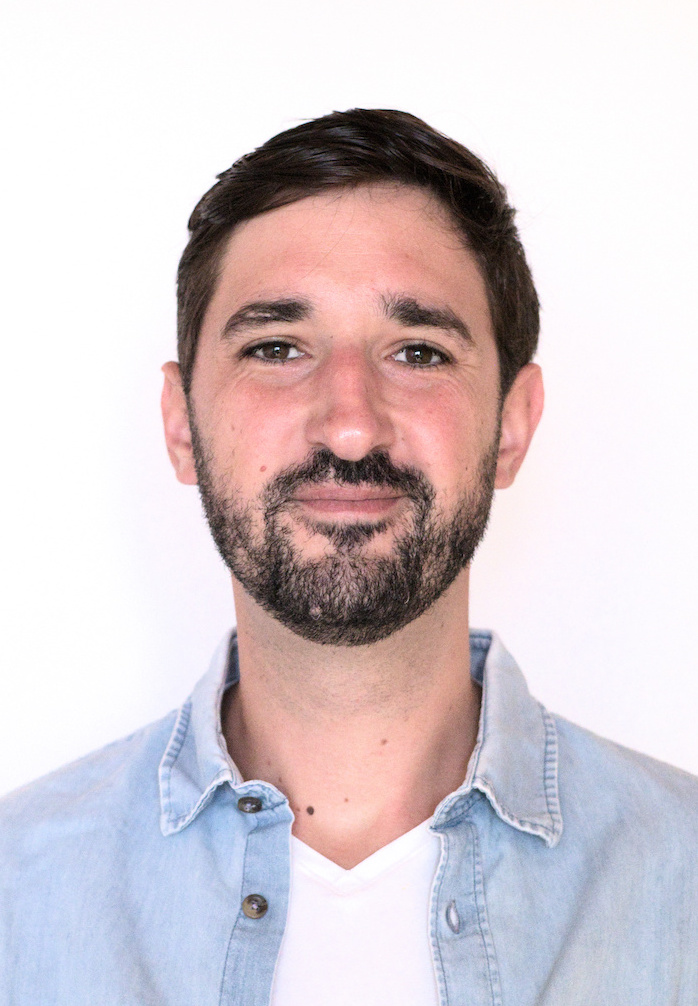
\includegraphics[width=\linewidth]{portrait_freehand.jpg}%
  \vspace{0.1em}
\end{minipage}

\cvsection{Strengths}

  \begin{tabularx}{\textwidth}{>{\scshape}l@{\hskip 3.5mm}L}
    Leadership & Mentoring, Recruiting, Budgeting, Performance Evaluation, Personal Development, Resource Allocation, Agile, Scrum\\
    Product Management & Vision, Design, Stakeholder Management, Forecasting, Market Study, Competition Analysis, Project Management, Risk Analysis, Roadmapping, Requirement Engineering\\
    Industrial IoT Design & Mechanics, Electronics, Firmware, QA, DFM, Supplier Management\\
    Backend Interfaces & AWS IoT Core, FleetHub, MQTT, Cloudwatch,  Lambdas\\
    Connectivity & 4G, 5G, Bluetooth, Bluetooth LE, LoRa\\
    Languages & French (Native), English (Business), German (Casual), Spanish (Basic)
  \end{tabularx}

\cvsection{Career}

  \makecareersubsection[0em]{Konux}{Railway Monitoring \& Predictive Maintenance}
    {Hardware Engineering Project \& Team Lead}
    {Aug. 2019 - Present}
    {Munich, Germany}{https://konux.com}

  \begin{tabularx}{\textwidth}{>{\scshape}l@{\hskip 3.5mm}L}
    Summary & Hiring \& Leading an Agile team of 11 professional engineers (primarily Senior Engineers).
    \par Hardware Product Vision, Portfolio \& Backlog for 4 independent products.
    \par Driving Product Acceptance and Technical reviews directly with Customers.
    \par Managing external development partners, suppliers, and manufacturing partners.
    \par Supporting Company Growth from $\sim 40$ to $\sim 120$ employees despite Covid.\\
    Tech. Stack & NXP, Nordic Semiconductors, Analog Devices, Bare metal, Zephyr RTOS, GNSS, 3G/4G/5G, BLE, Test Automation, Python, Jenkins, TestRail, AWS IoT Core, S3, Fleethub, Cloudwatch, Lithium Battery\\
    Materials &  Aluminium, (Stainless) Steel, Glass-fibre reinforced Plastics, PE, HDPR, Acrylic\\
    Standards & ISO 9001, European EMC \& RED, EN 50125, UN 38.3, RoHS\\
    Markets & Europe, North America, Asia-Pacific\\
  \end{tabularx}

  \begin{minipage}{\textwidth}
    \small
    I have the pleasure of leading an agile team of eleven exceptional electronics, mechanics, embedded software and QA engineers, as well as full-stack and backend developers. Together, we built a strong and efficient cross-functional product engineering team and took ownership of the entire lifecycle of our hardware portfolio and the backend interfaces they rely on. I provide the team with a hardware and software vision and roadmap (1-2 years ahead) as well as extensive product backlogs. Then, I accompany them through concept, design, prototyping, execution and validation until the final deliveries to our manufacturing partners. At the company level, I represent our hardware engineering efforts and ensure alignment with our Product, Sales, Customer Success, as well as Operations teams. I am thrilled to be able to mentor each individual contributor, both on technical aspects and personal growth.
  \end{minipage}
  

\makecareersubsection{Proglove}{Industrial wearables}
  {Hardware Engineering Team Lead}
  {Oct. 2017 - Jul. 2019}
  {Munich, Germany}{https://proglove.com}

  \begin{tabularx}{\textwidth}{>{\scshape}l@{\hskip 3.5mm}L}
    Summary & Hiring \& Leading a Scrum team of 13 professional engineers (all levels of seniority).
    \par Focus on one Wearable Product development with critical deadlines.
    \par Specified and Certified for International Markets.
    \par Internal and External Customer Management. 
    \par Introduce OKR methodology.
    \par Growth from Start-up to Successful Scale-up\\
    Tech. Stack & Nordic Semiconductors, Zephyr RTOS, BLE, Sub-GHz Radio, USB, Test Automation, Python, Lithium Battery\\
    Materials & Plastics\\
    Standards & European EMC \& RED, FCC (ID: : 2AOJL-MARK-2), IC (ID: 23450-MARK2), UL 62368, RoHS\\
    Markets & Europe, North America\\
  \end{tabularx}

  \vspace{1.5em}
  
  \begin{minipage}{\textwidth}
    \small
    Joining a young and dynamic team of electronics and embedded software developers as a validation engineer, I quickly took on the role of team lead as our need to develop a new product became a financial imperative for the company. Growing the team evenly from 5 to 13 engineers over the course of 18 months enabled us, in March 2019, to release our most successful product in both Europe and North America while still being able to work on other innovation projects. ProGlove went on to become an extremely profitable company, with its lighthouse product being the device and technology I had the pleasure to pioneer.
  \end{minipage}



\makecareersubsection{Intel Corporation}{Modem Platforms \& Transcievers}
  {Pre-silicon Validation \& Verification Engineer}
  {Aug. 2011 - May 2017}
  {Munich, Germany}{https://intel.com}

  \begin{tabularx}{\textwidth}{>{\scshape}l@{\hskip 3.5mm}L}
    Summary & SW/HW Test Automation for Pre- \& Post-Silicon Validation (automation).
    \par SW Architecture \& Infrastructure \& Methodology (White/Black Box Testing).
    \par Agile Project \& Software lifecycle management. 
    \par Stakeholder Management, Scheduling \& Resource Allocation.\\
    Tech. Stack & Python, LabView, Matlab, C/C++, 3G/4G Modem, Bluetooth, SMARTi transceiver, XMM Modem\\
    Locations & Europe, North America, India\\
  \end{tabularx}

  \vspace{1.5em}
  
  \begin{minipage}{\textwidth}
    \small
    Starting in 2011 as a validation and verification engineer, and later completing my Master's thesis within the Analog Design department, I took an interest in refining and streamlining our pre-silicon and post-silicon validation pipelines, leading me to join the embedded software verification team within the transceiver design department. In 2015, I enlisted the help of a scrum master, combining multiple software and hardware engineers distributed across Europe and the United States to solve a unique challenge in the semiconductor world: how to build a test automation system where emulation and real hardware can be validated using the same test vectors and test cases.
  \end{minipage}

\clearpage
    
\cvsection{Degrees}

  \makeeducationparagraph{Master of Science}{Microelectronics \& Telecommunications}
    {École d'Ingénieurs CPE Lyon}
    {2010 - 2013}{France}

  \makeeducationparagraph{Master's Thesis}{Comparison methodology of PLLs and Oscillators for transceiver designs}
    {Intel Corporation}
    {2013}{Germany}

  \makeeducationparagraph{Bachelor of Science}{Electronics \& Telecommunications}
    {École d'Ingénieurs CPE Lyon}
    {2007 - 2010}{France}


\cvsection{Outside of Work}

  \makehobbyparagraph[0em]{Ultralight Outdoor Equipment Design \& Manufacturing}
  {\href{https://abcpacks.com}{ABC Packs}}
  {
    For the last 7 years, I have regularly designed various types of backpacks and rucksacks with the goal of massively reducing the weight and volume of outdoor equipment one can carry on treks, expeditions, ski touring, etc. I take orders, design unique pieces of equipment - sometimes with the customer - then manufacture, ship and bill my creations.
  }
  
  \makehobbyparagraph{Hand-tool Woodworking \& Furniture Making}
  {}
  {
    I find wood to be a fascinating material to shape and build with. The steep learning curve requires a lot of patience and repetition to build muscle memory. After about 4 years of practice, I am only now starting to feel comfortable designing more complex and ambitious pieces of furniture. Yet, I still have a long road ahead of me.
  }

  \makehobbyparagraph{Long Distance Hiking \& Solo expeditions}
  {}
  {
    I set out on solo treks for weeks at a time in the Himalayas and in Swedish Lapland, and enjoy the European Alps from France to Romania for any length of time. I can also walk the Great Glen Way (125 km) in 4 days although I might need a few days to recover afterwards.
  }

  \makehobbyparagraph{Outdoor \& Street Photography}
  {}
  {
    My journey into photography started about 15 years ago. During that time, I shot both film (mostly 35mm) as well as many variations on digital cameras (DSLRs, mirrorless). I simply enjoy the process of creating a still image of a slice of life, taking time to compose an image that can resonate with someone else. I primarily gravitate around street \& travel photography though I have covered the occasional wedding.
  }

\end{document}